%%%%%%%%%%%%%%%%%%%%%%%%%%%%%%%%%%%%%%%%%%%%%%%%%%%%%%%%%%%%
% Document settings
\documentclass{ACGSeminar}

%%%%%%%%%%%%%%%%%%%%%%%%%%%%%%%%%%%%%%%%%%%%%%%%%%%%%%%%%%%%
% Own Packages
\usepackage{listings}
\usepackage{fancyhdr}

%%%%%%%%%%%%%%%%%%%%%%%%%%%%%%%%%%%%%%%%%%%%%%%%%%%%%%%%%%%%
% Own Definitions
\newcommand{\comment}[1]{}

%%%%%%%%%%%%%%%%%%%%%%%%%%%%%%%%%%%%%%%%%%%%%%%%%%%%%%%%%%%%
% BibTex
\bibliography{references}

%%%%%%%%%%%%%%%%%%%%%%%%%%%%%
% Hyphenations here
%%%%%%%%%%%%%%%%%%%%%%%%%%%%%
\hyphenation{Sa-tan-arch-aeo-li-deal-co-hell-ish}

%%%%%%%%%%%%%%%%%%%%%%%%%%%%%
% Title, Author, etc.

\pagestyle{fancy}
\fancyhf{}
%\rhead{}
%\lhead{\leftmark \rightmark}
\fancyhead[R]{\nouppercase{\leftmark}}
\fancyhead[L]{\nouppercase{\rightmark}}
\fancyfoot[C]{\thepage}

\begin{document}

\title{Re: Deep G-Buffers for Stable Global Illumination Approximation}

\author{Ferit Tohidi Far}

\maketitle

%%%%%%%%%%%%%%%%%%%%%%%%%%%%%%%%%%%%%%%%%%%%%%%%%%%%%%%%%%%%
% Abstract

\begin{abstract}%
G-buffers can be used to efficiently render images with large amounts of light sources. This is possible thanks to a process called "deferred rendering". Using 
only g-buffers, we are only able to compute local illumination, which forces us to find a way to achieve sought after visual and lighting effects like global 
illumination. By using deep g-buffers we can approximate global illumination in a way that is more efficient than traditional methods like pathtracing, 
while of course not being physically accurate. We can make up for it, though, by also approximating visual effects like ambient occlusion, color bleeding, reflections, 
depth of field and motion blur to create an acceptable interactive realtime result, which is - as of now - simply impossible with physically accurate methods on 
average hardware.
\end{abstract}

\keywords{nvidia, g-buffer, deep g-buffer, pathtracing, global illumination approximation, deferred shading, deferred rendering}
\tableofcontents
\listoffigures
\listofalgorithms

\label{cha:references}

\newpage

%%%%%%%%%%%%%%%%%%%%%%%%%%%%%%%%%%%%%%%%%%%%%%%%%%%%%%%%%%%%
% Introduction
\label{cha:introduction}
\section{Global illumination}
	In order to understand why computing global illumination is such a big deal, we first need to set the stage by introducing the essentials of traditional rendering. Global illumination is a lighting effect that is achieved by not only computing direct light, but also indirect light, meaning that it is neccesary to take	into account how light reflects and carries information (in the most basic case: color). On the contrary, local illumination is computed by only considering direct light, meaning that the resulting image will lack details and visual effects that would otherwise convey realism. These visual effects are ambient occlusion, color bleeding, reflections, caustics, and soft shadows. What all these visual effects describe is explained in section 4.
	\subsection{Physically correct methods}
	In order to generate physically correct lighting, which is a requirement for creating photorealistic images, we need to solve the rendering equation
	$$ L_o(\omega) = L_e(\omega) + \int_\Omega f(\omega, \omega')L_i(\omega')cos(n, \omega') \partial \omega' $$
	where 
	\begin{center}
		\begin{align*}
			&L_o(\omega) \text{ is the outgoing light in direction } \omega\text{,}\\
			&L_e(\omega) \text{ is the emmited light in direction } \omega\text{,}\\
			&f(\omega, \omega') \text{ is the BRDF\footnotemark} \text{,}\\
			&L_i(\omega') \text{ is the incoming light from direction } \omega'\\
			&\text{and } cos(n, \omega') \text{ is lambert reflectance\footnotemark}  \text{ .}
		\end{align*}
	\end{center}
	\addtocounter{footnote}{-1}
	\footnotetext{The bidirectional random distribution function basically describes the reflection/refraction of a ray on surface.}%
	\stepcounter{footnote}
	\footnotetext{Lambert reflectance describes the attentuation of light on diffuse objects based on the lights incident angle.}%
	The most popular method for achieving this is pathtracing \cite{P2PATH}.
	\subsubsection{Pathtracing}
		solves the rendering equation by first sending camera rays through each individual pixel of the image plane and then tracing the ray back to the light source. If the lamp is hit the pixel gets painted painted with color, else black. Direct consequences of this are soft shadows and ambient occlusion. A maximum hop number caps the amount of times a ray is able to reflect. A hop number larger than 1 (3 in most simple cases is sufficient, but it is dependent on the complexity of the scene) allows for global illumination. The reflections and refractions are essentially determined by the BRDF, which not only means that objects can be transparent, but we also get caustics\footnote{Caustics are areas with concentrated light. This happens due to light refracting.}. With each surface a ray hits it carries information from that surface, e.g. its color, and reflects it onto the next surface it hits. This causes color bleeding. Each pixel is sampled thousands - possibly hundreds of thousands - of times to reduce the noise that is induced by diffuse reflections, resulting in a photorealistic render.
	\subsection{Computational difficulties of physically correct methods}
	Since we have to take into account thousands of samples of every ray of light with its reflections, the computational difficulty becomes apparent \cite{DST}. Because of this, it is nearly impossible to achieve real time rendering using physically correct methods on an average system. This forces game engines to stick to \textbf{faking} global illumination and visual effects since it is way more efficient to compute. Adding multiple light sources to the scene will still be challenging to average systems with traditional rendering (forward rendering) as described by modern graphics pipelines. Deferred rendering, specifically deferred shading, counters this problem at the cost of having to compute transparency using depth peeling and having no straight forward anti-aliasing.
	%TODO explain anti-aliasing and why there is no support with deferred rendering

\section{Deferred rendering}
	Graphics pipelines describe each step that has to be taken in order to render an image. Within a pipeline it is possible in some cases to defer steps to a later stage. It is conventional to use GPU's for applications that rely heavily on rendering images. There is no universal graphics pipeline, because these are dependent on the GPU that is used, which means it is convenient that there exist API's like OpenGL that try to generalize the steps that need to be taken in order to render an image and map them to compatible GPU's. This means that most GPU dependent applications abide by the graphics pipeline as described by, for instance, OpenGL (figure \ref{fig:graphics_pipeline}).
	\begin{figure}[htb!]%
	\begin{center}%
		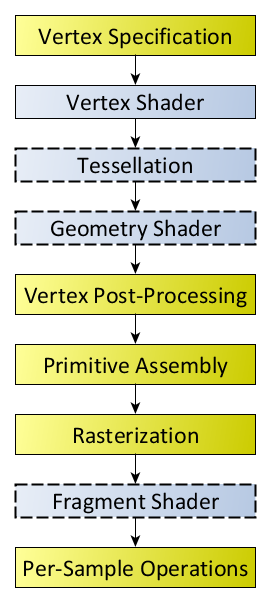
\includegraphics[height=7cm]{img/graphics_pipeline.png}
	\end{center}%
	\caption{The OpenGL graphics pipeline. All steps are mandatory, but the ones within blue boxes are also programmable and the ones with dashed borders can be deferred or forwarded. Note that the vertex-shader and geometry-shader do not neccesarily compute any shading or colors, but can be programmed to do so. They are called shaders for historical reasons, which might be a little irritating.}%
	\label{fig:graphics_pipeline}%
	\end{figure}%
	\subsection{How deferred shading handles lighting more efficiently}
		The goal of deferred shading is to defer the shading stage. 
		Instead of shading right away, we compute necessary geometry buffers (g-buffers) in a first pass that we call "geometry pass" and cache 
		them for later use in the second pass which we call "shading (or lighting) pass". With forward rendering we would have to compute the shading for every fragment of every object for all light-sources in a single pass. The shading is applied regardless wether the fragment is visible at the end or not, since the visibility test is performed at the end. This means that the time complexity of computing forward shading is $O(amount_{fragments} \cdot amount_{lights})$. If we apply deffered shading, however, we do not force ourselves to shade every fragment as soon as it has been computed, instead we wait until we find the closest fragment so to say. Finding the closest fragment is called "solving the visibility problem". This is solved during the geometry pass when filling the z-buffer with its respective z-values, which can be computed by performing perspective correct interpolation between the vertices of the current polygon (in most cases triangles). The z-buffer, along with all other buffers that are collected, are continuously updated if a closer fragment for the same pixel is found, which solves the visibility problem. Now all the fragments that we shade are only going to be shaded once, which means for the time complexity that the shading is done in $O(amount_{pixels} \cdot amount_{lights})$, allowing us to render more light-sources at the expense of passing around g-buffers (note that fragments are \textbf{potential} pixels). For all practical purposes, g-buffers have to at least consist of a frame-buffer, a normal-buffer and a z-buffer. Using only these g-buffers, it is possible to render an image with basic shading.

\section{Geometry-buffer (g-buffer)}
	Each geometry-buffer stores information of some sort for each individual pixel, meaning that they are all two-dimensional arrays using the dimensions of the screen. Note that there are more possible buffers to choose from, but the three that will be mentioned are the most essential in every g-buffer.
	\subsection{Frame-buffer}%
		Color-values of fragments are stored in the frame-buffer. It basically stores the rendered image without fragment-shading\footnote{Fragment-shading (also called pixel-shading) aims to shade every single fragment by using some shading technique phong-shading.} applied to it.% 
		\begin{figure}[htb!]%
			\begin{center}%
				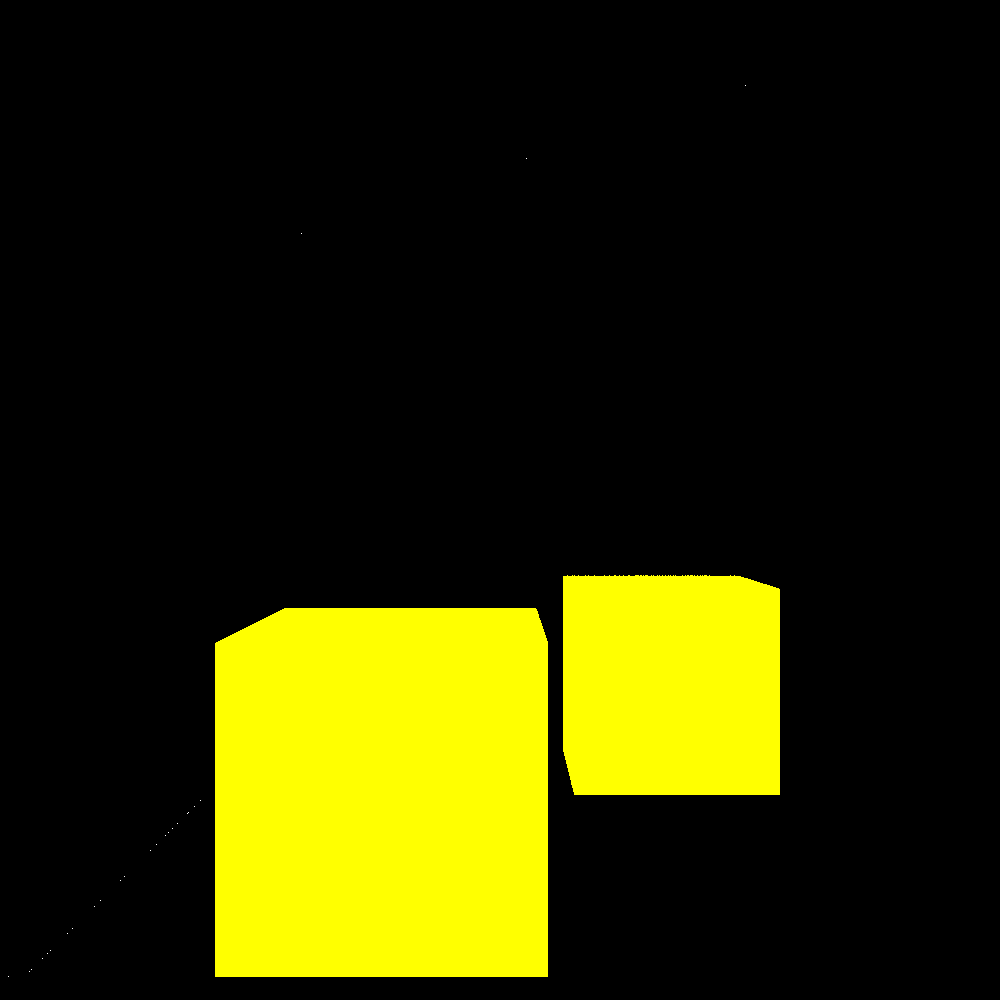
\includegraphics[width=7cm]{img/frame_buffer.png}
			\end{center}%
			\caption{Example of a frame-buffer (also called image-buffer). It shows a cornell box with pitch black walls containing two yellow cuboids.}%
			\label{fig:frame_buffer}%% TODO update this figure ...
		\end{figure}%
	\subsection{Z-buffer}
		The z-buffer stores depth values of fragments. These are needed to determine which surfaces are closest and visible to the camera. If two different fragments\footnote{A fragment is a point on a surface in worldspace\footnotemark} have the same x and y coordinates in screenspace\footnotemark, then the fragment with the smaller z-value is supposed to be in front of the other. This buffer is also used for screenspace visual effects like screen space ambient occlusion and depth peeling. 
		\addtocounter{footnote}{-1}
		\footnotetext{Worldspace is the space in which the 3d objects are placed.}
		\stepcounter{footnote}
		\footnotetext{Screenspace is the space in which the individual pixels of the projected 3d models are defined.}
		\begin{figure}[htb!]%
			\begin{center}%
				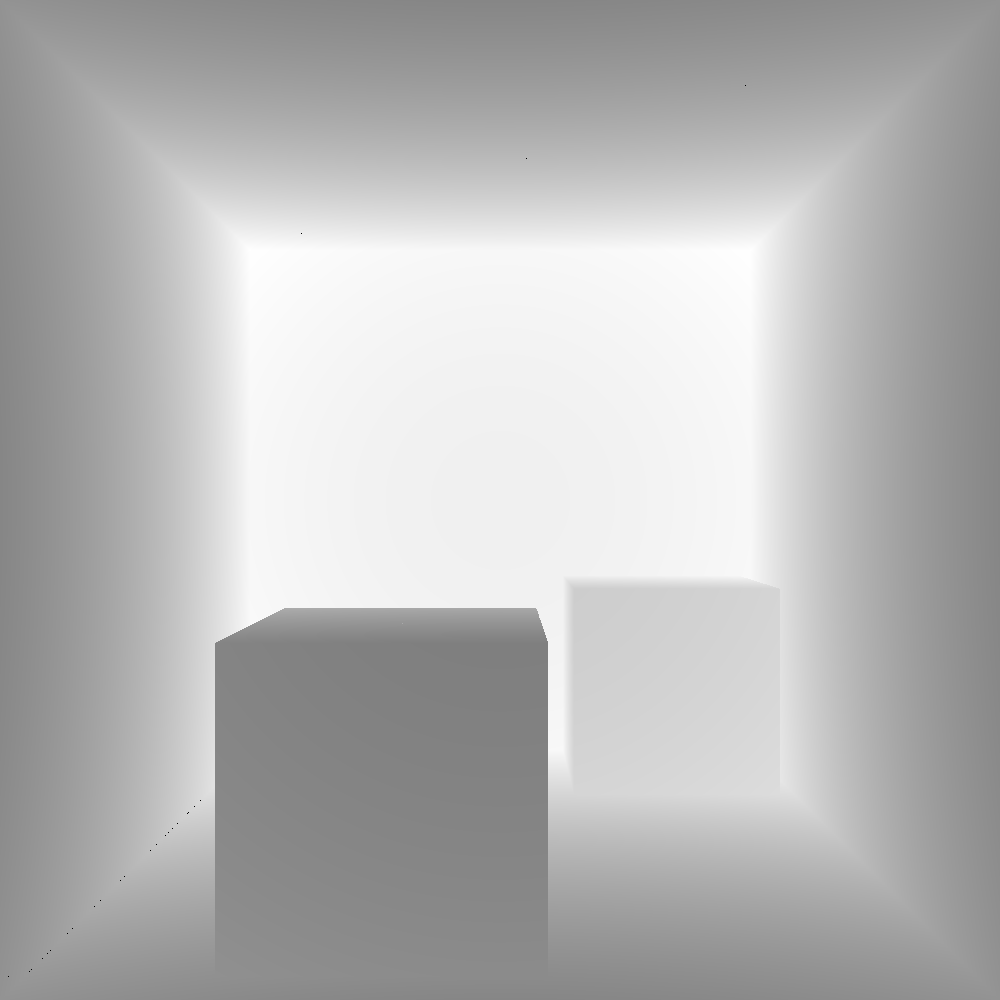
\includegraphics[width=7cm]{img/z_buffer.png}
			\end{center}%
			\caption{Example of a z-buffer. Since the z-buffer only stores distances as float values instead of actual colors they are interpreted as the grayscale value deduced by dividing each
			z-value by the distance of the furthest away object from the cameras point of view, which is the maximum z-value, and then multiplying with 255 to create an RGB color vector.}%
			\label{fig:z_buffer}% TODO update this figure ...
		\end{figure}%
	\subsection{Normal-buffer}
		The normal-buffer stores surface-normals that are mostly used to determine reflection and refraction directions. They are also used for light attentuation, since they help determine the cosine of the surface and the incident light and a larger cosine means lighter light and vice versa (lambert reflectance).
		\begin{figure}[htb!]%
			\begin{center}%
				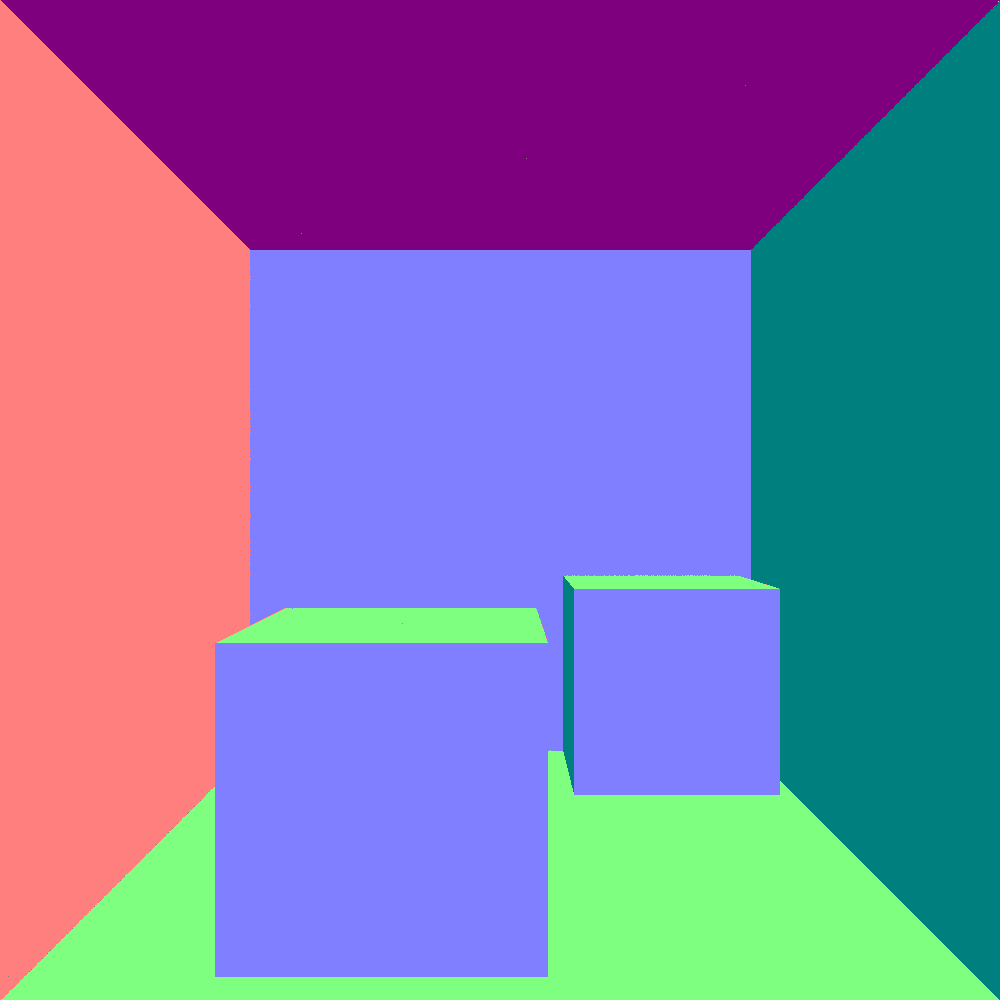
\includegraphics[width=7cm]{img/normal_buffer.png}
			\end{center}%
			\caption{Example of a normal-buffer. Normal vectors in this buffer are normalized, meaning their component values range from -1 to 1. Since negative normals would cause negative RGB values, we add $(1, 1, 1)$ and scale with $255/2$, which results in a usable RGB color.}%
			\label{fig:normal_buffer}%% TODO update this figure ...
		\end{figure}%
	\subsection{Computing local illumination using g-buffers (deferred shading)}
		After having collected all our g-buffers we can now work on local illumination. To do this we need to define some light sources. The following are some of the possible light-sources that we can use:
		Point-lights, spot-lights and directional-lights \cite{DST}. The simplest one is directional-light. We simply specify an origin in worldspace from which the light rays are sent in all directions. A point-light is a directional-light which is constrained by its radius (basically a sphere of light). Finally, spot-lights are area lights which emit light on another area (like spot-lights in real life do). 
		At this point we have to choose a shading technique. The most popular ones are gouraud-shading and phong-shading. The differences are essentially that gouraud-shading assigns shaded colors to the vertices of a polygon within the vertex-shader and then interpolates (blends) the colors inbetween the vertices in the fragment-shader, while phong-shading directly computes the shaded colors for each individual fragment in the fragment-shader. Gouraud-shading is a fast way of computing shading since interpolating between three (assuming the polygons are triangles) shaded vertices is quicker than actually computing a color by considering the light sources for each individual fragment as is done by phong-shading, but may look edgy if the 3d models are made of few polygons, which would make phong-shading preferable in that case.

\section{Visual effects} \label{visual_effects}
	The following are visual effects that are sought after, but some of them are hard or impossible to achieve physically correct without using
	computationally expensive methods. When applying pathtracing, we get most of the following effects for free: 
	\begin{figure}[htb!]%
	\begin{center}%
		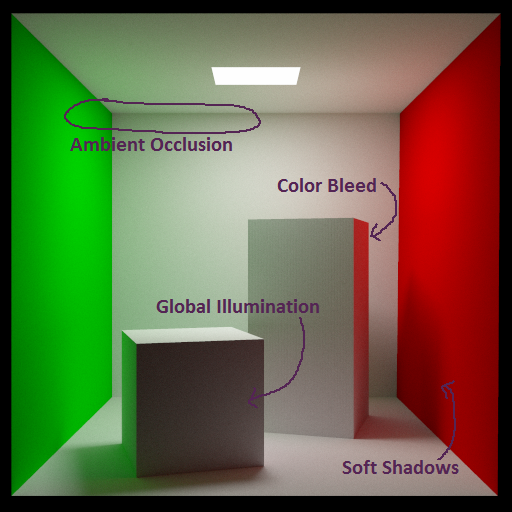
\includegraphics[width=7cm]{img/visual_effects.png}
	\end{center}%
	\caption{Diverse visual effects caused by global illumination inside a cornell box. The image was rendered using pathtracing.}%
	\label{fig:visual_effects}%
	\end{figure}%
	\subsection{Ambient occlusion}
		Ambient occlusion essentially describes how much shading the "in-betweens" of a 3d object gets. This effect can be efficiently approximated by using a method called - ironically - screen space ambient occlusion (SSAO). This method basically runs an edge detector over the z-buffer and paints those edges black. Since it only runs over the z-buffer it is considered screen space. Since ambient occlusion is an effect directly caused by global illumination, the method (ambient occlusion) is considered an efficient way of faking global illumination.
		\begin{figure}[htb!]%
			\begin{center}%
				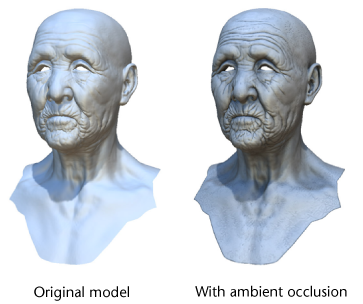
\includegraphics[width=7cm]{img/ambient_occlusion.png}
			\end{center}%
			\caption{How ambient occlusion affects the realism of a rendered 3d model. The "in-betweens" of the model appear to have depth.}%
			\label{fig:normal_buffer}%
		\end{figure}%
	\subsection{Color bleeding}
		Color bleeding happens when light directs information from one hit-surface to another. Let A and B be objects. If A reflects light onto B and A's surface is blue, then B will also appear
		to be slightly blue on the reflected area. To have this happen it is obviously necessary to trace rays of some sort. This can be approximated, though, using ... %TODO how is this approximated?

	\subsection{Soft shadows}
		We can easily compute hard shadows using shadow mapping. This is done by projecting the scene from the light source's point of view and then projecting the scene from the camera's point of view while only actually painting the points with their respective colors if they are hit by light, else they are painted black. To get soft shadows, the points in shade simply get blended together with their surrounding points.

	\subsection{Transparency}
		A quick method to achieve transparency is depth peeling. To do this we need two g-buffers at a time ...\cite{NOIT}.
		%TODO explain depth peeling

	\subsection{Reflection}
		Screen space mirror reflections can be efficiently computed through environmental mapping (also called reflection mapping). This is done by projecting the texture that is supposed to be reflected onto the object that reflects it.
		%TODO be more precise about this

	\subsection{Depth of field}
		Depth of field ...
		%TODO explain depth of field

	\subsection{Motion blur (in interactive applications)}
		Motion blur ...
		%TODO explain motion blur

\section{Deep g-buffer}
	Deep g-buffers make use of a concept similar to depth peeling. Instead of storing information about the closest surface, in an n-layer deep g-buffer we also store information about the n-closest surface \cite{NDGB}. This means we store g-buffers for the closest surfaces, then the second-closest surfaces and eventually the n-closest surfaces in an n-layer deep g-buffer. Practical observations suggest that the second-closest surface is often not the second-most relevant for shading and visual effects \cite{NDGB}. To resolve this issue we rely on minimum depth separation, which essentially introduces a distance $\Delta z$ that has to be exceeded when looking for the next-closest surface immediately after the current one.
	\subsection{Generating a 2-layer deep g-buffer}
		NVIDIA proposes two ways of generating a 2-layer deep g-buffer, one of which is straight forward to help demonstrate the idea and one of which is efficient. The first one they call "Strawman Two-Pass Generation Algorithm":
		\begin{algorithm} \label{alg:two_pass_strawman} \caption{Two pass strawman algorithm for generating 2-layer deep g-buffers}
		\begin{lstlisting}[frame=single]
//1st pass
submit geometry with:
  geometryShader(tri):
    emit T(tri) to layer 0
  pixelShader(x, y, z):
    return S(x, y, z)

//2nd pass
submit geometry with:
geometryShader(tri):
    emit T(tri) to layer 1
  pixelShader(x, y, z):
    if z > Z[0][x][y] + \Delta z:
      return S(x, y, z)
    else:
      discard fragment
		\end{lstlisting}
		\end{algorithm}
		where $Z$ is the 2-layer z-buffer and $S(x, y, z)$ returns other g-buffers needed for shading. Since fragments get discarded if their distance to the previous fragment is smaller than $\Delta z$ the minimum depth seperation constraint is met. However, there is a more efficient algorithm which only requires a single pass: 
		\begin{algorithm} \label{alg:one_pass_strawman} \caption{An improved one-pass algorithm for generating 2-layer deep g-buffers}
		\begin{lstlisting}[frame=single]
submit geometry with:
  geometryShader(tri)
    emit T(t, tri) to layer 0
    emit T(t, tri) to layer 1
  if VARIANT == Delay) or (VARIANT == Predict:
    emit T(t+1, tri) to layer 2
  pixelShader(x, y, z):
    switch (layer):
      case 0: // 1st layer; usual G-buffer pass
        return S(x, y, z)
      case 1: // 2nd G-buffer layer: choose the comparison texel
        if VARIANT == Delay) or (VARIANT == Predict:
          L = 2 // Comparison layer
          C = (x, y, z) // Comparison texel
        else if VARIANT == Previous:
          L = 0; C = (x, y, z)
        else if VARIANT == Reproject:
          L = 0; C = (x[t-1] , y[t-1], z[t-1])
        if z C > Z[t-1] [L][x[C], y[C] ] + delta_z: return S(x, y, z)
        else: discard the fragment
      case 2: // Depth only write to predict Z[t+1][0]; no shading
        return // We only reach this case for Delay and Predict
		\end{lstlisting}
		\end{algorithm}
		where $t$ is the frame-index 
	\subsection{How deep g-buffers approximate visual effects}
	\subsubsection{Global illumination} 
		is achieved by ...
	\subsubsection{Ambient occlusion}
		blabalbal ...

\section{Deep g-buffers vs pathtracing: Global illumination}
\section{Conclusion}
	Deep g-buffers seem to do a good job at faking global illumination in real time. In the future deep g-buffers are going to be used for ...

%%%%%%%%%%%%%%%%%%%%%%%%%%%%%%%%%%%%%%%%%%%%%%%%%%%%%%%%%%%%
% Bibliography
\printbibliography

\end{document}